\documentclass{article}


% Packages
\usepackage[utf8]{inputenc} % For Norwegian letters
\usepackage{tabulary} % For nice tables
\usepackage{multirow}
\usepackage{graphicx}
\usepackage{caption}
\usepackage{subcaption}
\usepackage{float}

% Config
\setlength{\parindent}{0cm} % Removes paragraph indentation
\setlength{\parskip}{1em} % Adds paragraph vertical skip

\newcolumntype{Y}{>{\centering\arraybackslash}X}
\renewcommand{\arraystretch}{2}

\begin{document}

% Title
\title{\textbf{Module 6} \\ IT3105}
\author{Magnus Gundersen, Simon Borøy-Johnsen \\ MTDT}
\date{\today}
\maketitle
% End Title


% Content
\section{ANN design}
Based on our experience with module 5, we tried hidden layers with around 500 nodes. This did not work very well. By trial and error we got to three hidden layers, one with 160 nodes, one with 320 nodes, and one with 160 hidden nodes. 

\begin{tabular}{|l|l|l|l|}
    \hline
    Hidden layers     & Topology            & Activation functions          & Learning rate  \\\hline
    3                 & [160, 320, 160]     &   [T.tanh, T.tanh, T.tanh]    & 0.01             \\\hline              
\end{tabular}

The function tanh() was chosen because, by trail and error, it gave us the best results. The learning rate was adjusted to fit the size of the training set, as this was expanding throughout the development of our system.

\section{Pre-Processing}

The first pre-processing of the data we tried was to square all the entities in the input board. This was done to in an attempt to make the ANN recognize the same shape with different values, by making the difference between different tiles higher than it usually is. This also emphasised the significance of having higher tiles, which is the goal of the game.

The second pre-processing we tried was to emphasise the snake-heuristic used in the generated training data. This was done by matrix-multiplication of the input-board and a static 4x4 matrix. The upper left corner in the matrix contained the highest value. Then, the values decreased along the pattern shown in figure \ref{fig:pattern}. This was done to make the ANN recognize the snake formation, to facilitate and emphasise different types of board configurations with the same shapes, but different tile values.

\begin{figure}[H]
    \centering
    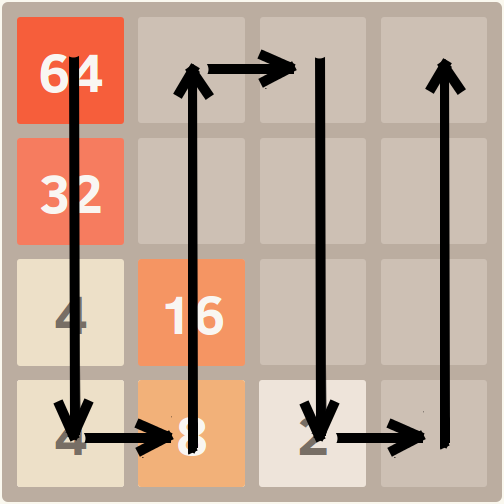
\includegraphics[scale=0.45]{images/path.png}
    \caption{Snake pattern}
    \label{fig:pattern}
\end{figure}

We ran each of the representations 50 times. We recorded the average value of the highest tile, and the average number of points the runs would yield at demo day. 

\begin{tabular}{|l|l|l|l|}
    \hline
    Representation no.   & Properties            & Avg. high tile     & Avg. points    \\\hline
    1                   & Squaring              &  208.67           & 6.9           \\\hline   
    2                   & Snake                 &  166,40           & 5.6           \\\hline    
\end{tabular}

We can see that the first representation is by far the best one. It has a significantly better expected outcome. We therefore chose the first representation. This is backed by the Welsh's T test's (rep1, rep2) p value: 0.147, that states that there indeed is a significant difference in the data sets.

The reason we only looked at the average high tile and average demo score is very simple. We are only interested in knowing how good the ANN can perform, and consequently, how many points we can score on this module. As other data (training accuracy etc.) is not relevant to these two points, we have left them out of the report. 

\section{Analysis of a game}

The ANN did not achieve very good results when playing the game, at least compared to the AI-solver from module 4. We used the best performing ANN; using the topology described with representation one. 

We can see that the ANN can efficiently learn to place the highest tiles in the leftmost column. This can be seen in the figure below.

\begin{figure}
\centering
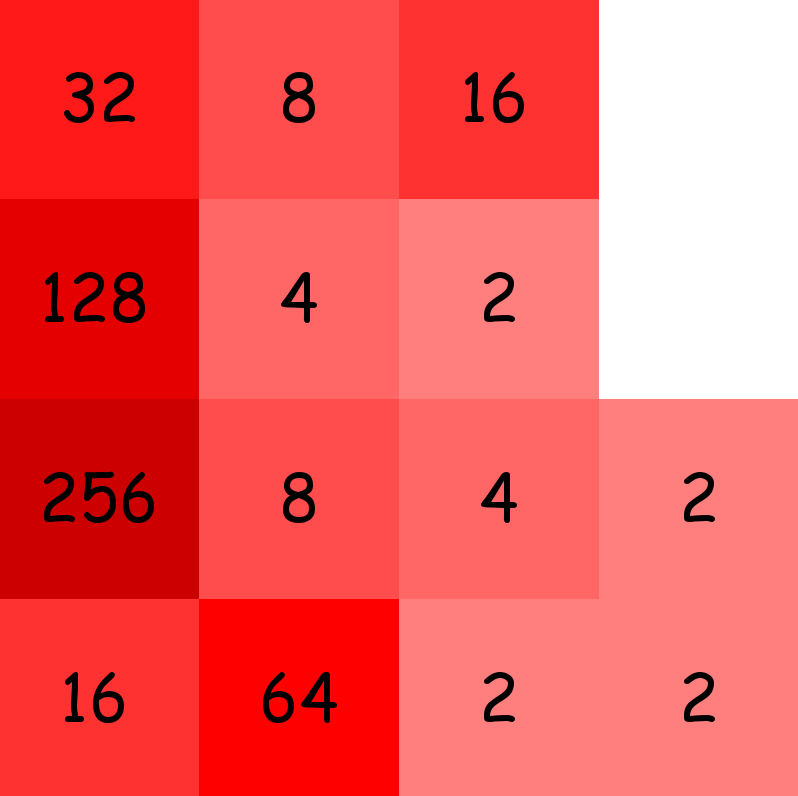
\includegraphics[scale=0.2]{images/samling.png}
\caption{High tiles gathering}
\label{fig:my_label}
\end{figure}

We can also see that the ANN has learned that it should merge tiles. Many times during the execution of a game, the ANN chose to merge tiles as fast as possible. This is evident in figure \ref{fig:merging}

\begin{figure}[H]
\centering
\begin{subfigure}{.6\textwidth}
  \centering
  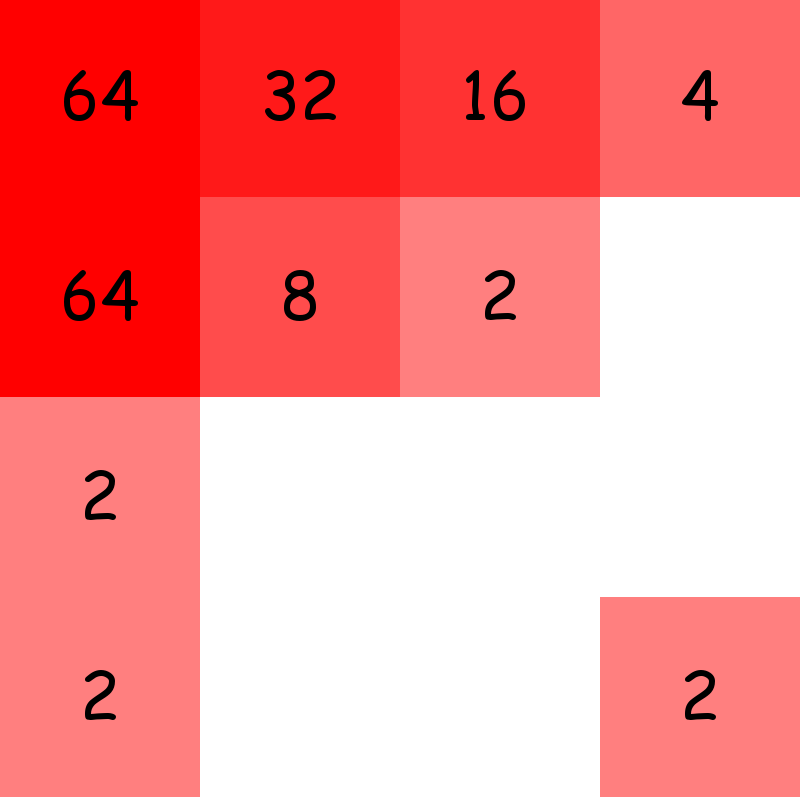
\includegraphics[width=.6\linewidth]{images/merge-before.png}
  \caption{Before merging}
  \label{fig:sub1}
\end{subfigure}%
\begin{subfigure}{.6\textwidth}
  \centering
  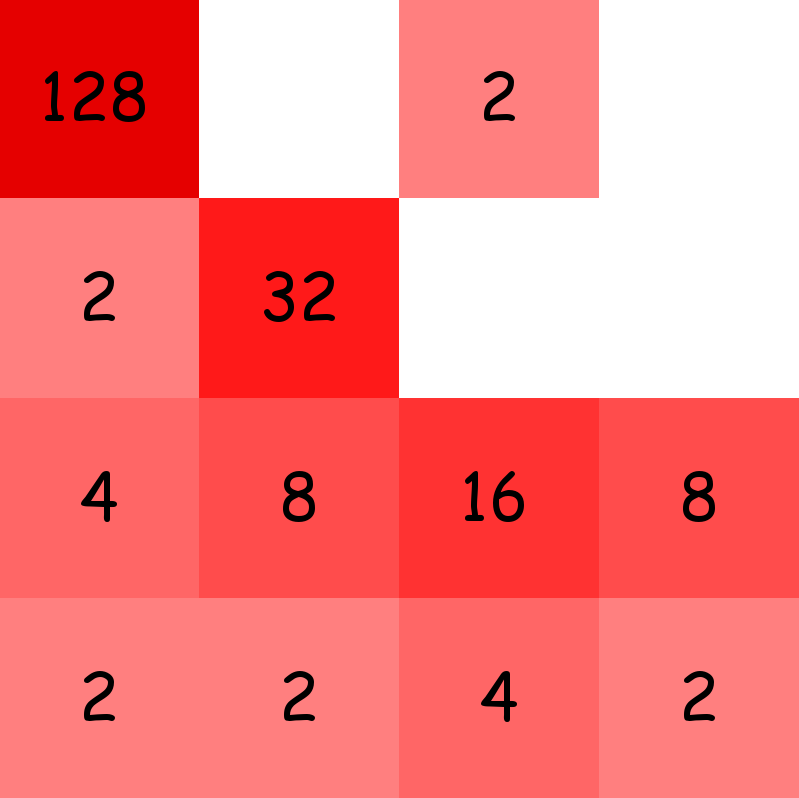
\includegraphics[width=.6\linewidth]{images/merge-after.png}
  \caption{After merging}
  \label{fig:sub2}
\end{subfigure}
\caption{The ANN merged the two 64-tiles, before continuing on as normal (with a down move)}
\label{fig:merging}
\end{figure}

However, we can also see that the ANN does not act in a way that it maximises the expected outcome in the future. This boils down to the fact that the majority of the board that the ANN encounter, is not in the training set. This means that the ANN will use what it has learned to maximise the short-term outcome.
% End content

\end{document}
